\documentclass[12pt]{article}
\usepackage{multirow}
\usepackage{tabularx}
\usepackage{graphicx}
\begin{document}

\title{Meal Planner Requirements Specification v1.0}

\author{
        Michael Kilian
}
\date{\today}

\maketitle
\tableofcontents



\newpage
\begin{abstract}
This document contains the identified requirements for the meal planner system. This document is subject to change as the project progresses. A minor version number change (e.g. 1.1 to 1.2) indicates the refinement of requirements. A major change (e.g. 1.2 to 2.0) indicates the addition or removal of requirements after they are identified through requirements elicitation.\\\\
For some use cases there are missing entries; this may be because further info is required to complete them, or it may be because the work flow is already obvious or dictated by the chosen framework (login is an example of such).
\end{abstract}
\newpage

\section{Domain Model \& Users}
%%%%%%%%%%%Domain Model%%%%%%%%%%%%%%%
\begin{figure}[h]
\caption{Users}
\centering
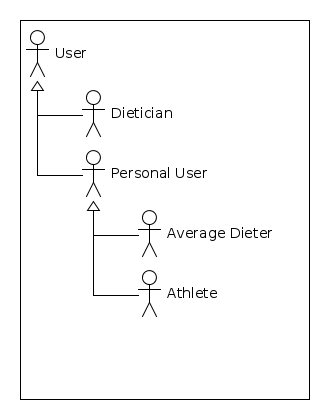
\includegraphics[width = 1\textwidth]{Users.png}
\label{fig:DomainModelUsers}
\end{figure}

There are three key user types identified in the domain. These are represented in Figure~\ref{fig:DomainModelUsers}.

\subsection{Personal Users}
As the name suggest, a personal user is anyone who uses the app for managing their own nutrition. They track their own goals and requirements only. This group can be further subdivided into two groups, dubbed Average Dieter and Athletes. These two groups will have very similar (possibly identical) interaction with the system. What differentiates the two is their domain knowledge and commitment.
\subsubsection{Average Dieter}
The Average Dieter group represents the average person looking to lose/gain weight or eat healthily. They will have fairly loose fitness goals, such as to simply lose some weight. As such for this user the exact distribution of nutrients in a meal is likely to be of lower importance compared to the total calories, the ease of preparing the meal and the palatability of the meal. They will likely have little to no knowledge of what constitutes good nutrition, so the app needs to support this by making some decisions for them by default to ensure their diet is 'healthy'. 

\subsubsection{Athlete}
In this context, the term athlete encompasses any user with very specific goals or users for whom correct nutrition is essential in supporting other activities. This could include runners, bodybuilders, footballers, etc. In contrast to the Average Dieter, the Athlete has specific goals and is likely to already have some understanding of nutrition. 


\newpage
\section{User Management}
%User Management encompasses user's interaction with their account

\subsection{Login \& Logout}

%%%%%%Login, Logout & Create New Account
\begin{figure}[H]
\caption{Login \& Logout}
\centering
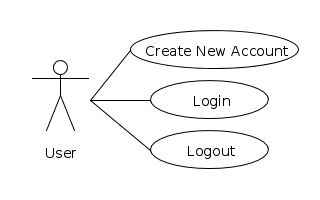
\includegraphics[width = 1\textwidth]{CreateNewAccount.png}
\label{useCaseDiagram:LoginOut}
\end{figure}

%%%%%%%%%%%%%%%%Create New Account %%%%%%%
\begin{center}
\begin{tabularx}{\textwidth}{ |X|X|}
\hline
\multicolumn{2}{|c|}{\textbf{Create New Account}}\\
\hline
\hline
\textbf{Use Case Diagram(s)} & Figure ~\ref{useCaseDiagram:LoginOut}\\ \hline
\textbf{Description} & User creates a new account, registering an email account and choosing a unique username and password.\\ \hline
\textbf{Process} & \\ \hline
\textbf{Scenarios} & \\ \hline
\textbf{Includes} & \\ \hline
\textbf{Extends} & \\ \hline
\textbf{Pre Conditions} & User has no account.\\ \hline
\textbf{Post Conditions} & User has an account registered.\\ \hline
\textbf{Rationale} & \\ \hline
\end{tabularx}
\end{center}


%Login 
\begin{center}
\begin{tabularx}{\textwidth}{ |X|X|}
\hline
\multicolumn{2}{|c|}{\textbf{Login}}\\
\hline
\hline
\textbf{Use Case Diagram(s)} & Figure ~\ref{useCaseDiagram:LoginOut}\\ \hline
\textbf{Description} & User logs in to system, giving them access to their account. \\ \hline
\textbf{Process} & \\ \hline
\textbf{Scenarios} & \\ \hline
\textbf{Includes} & \\ \hline
\textbf{Extends} & \\ \hline
\textbf{Pre Conditions} & User is not logged in.\\ \hline
\textbf{Post Conditions} & User is logged in, denied access, or quits.\\ \hline
\textbf{Rationale} & \\ \hline
\end{tabularx}
\end{center}

%Logout
\begin{center}
\begin{tabularx}{\textwidth}{ |X|X|}
\hline
\multicolumn{2}{|c|}{\textbf{Logout}}\\
\hline
\hline
\textbf{Use Case Diagram(s)} & Figure ~\ref{useCaseDiagram:LoginOut}\\ \hline
\textbf{Description} &  User logs out of system manually, or is logged out automatically after being inactive for a period of 15 minutes. \\ \hline
\textbf{Process} & \\ \hline
\textbf{Scenarios} & \\ \hline
\textbf{Includes} & \\ \hline
\textbf{Extends} & \\ \hline
\textbf{Pre Conditions} & User is logged in.\\ \hline
\textbf{Post Conditions} & User is logged out.\\ \hline
\textbf{Rationale} & \\ \hline
\end{tabularx}
\end{center}


\newpage
\subsection{Personal Statistics \& Goals}

%%%%%%%%%%%%%%Statistics, Calculations and Requirements %%%%%%%%%%%%%%
\begin{figure}[h]
\caption{Personal Statistics and Goals}
\centering
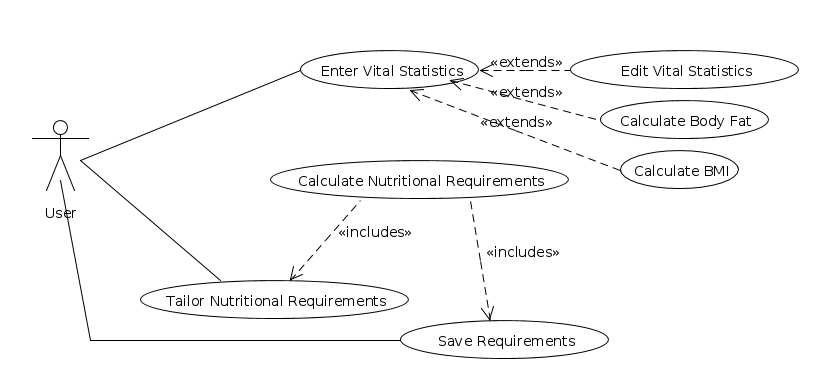
\includegraphics[width = 1\textwidth]{TailorAndSaveRequirements.png}
\label{useCaseDiagram:PersonalGoalsAndStatistics}
\end{figure}


%Enter vital statistics
\begin{center}
\begin{tabularx}{\textwidth}{ |X|X|}
\hline
\multicolumn{2}{|c|}{\textbf{Enter current vital statistics}}\\
\hline
\hline
\textbf{Use Case Diagram(s)} & Figure ~\ref{useCaseDiagram:PersonalGoalsAndStatistics}\\ \hline
\textbf{Description} & User enters the following vital statistics : height, weight , age and gender. They may also optionally enter body fat percentage.  \\ \hline
\textbf{Process} & \\ \hline
\textbf{Scenarios} & \\ \hline
\textbf{Includes} & \\ \hline
\textbf{Extends} & \\ \hline
\textbf{Pre Conditions} & Vital statistics are unknown. \\ \hline
\textbf{Post Conditions} & New vital statistics are saved.\\ \hline
\textbf{Rationale} & These statistics are used to calculate their requirements and track their progress towards weight loss/gain goals.\\ \hline
\end{tabularx}
\end{center}


%Edit Vital Statistics
\begin{center}
\begin{tabularx}{\textwidth}{ |X|X|}
\hline
\multicolumn{2}{|c|}{\textbf{Edit Vital Statistics}}\\
\hline
\hline
\textbf{Use Case Diagram(s)} & Figure ~\ref{useCaseDiagram:PersonalGoalsAndStatistics}\\ \hline
\textbf{Description} & Users updates their vital statistics to reflect changes over time. \\ \hline
\textbf{Process} & \\ \hline
\textbf{Scenarios} & \\ \hline
\textbf{Includes} & Enter Vital Statistics.\\ \hline
\textbf{Extends} & \\ \hline
\textbf{Pre Conditions} & User's vital statistics are known but out of date.\\ \hline
\textbf{Post Conditions} & New statistics are saved.\\ \hline
\textbf{Rationale} & Vital statistics change over time.\\ \hline
\end{tabularx}
\end{center}


%Calculate BMI
\begin{center}
\begin{tabularx}{\textwidth}{ |X|X|}
\hline
\multicolumn{2}{|c|}{\textbf{Calculate Body Mass Index}}\\
\hline
\hline
\textbf{Use Case Diagram(s)} & Figure ~\ref{useCaseDiagram:PersonalGoalsAndStatistics}\\ \hline
\textbf{Description} & Calculate the Body Mass Index of the user.\\ \hline
\textbf{Process} & \\ \hline
\textbf{Scenarios} & \\ \hline
\textbf{Includes} &  \\ \hline
\textbf{Extends} & Enter Vital Statistics. \\ \hline
\textbf{Pre Conditions} & \\ \hline
\textbf{Post Conditions} &\\ \hline
\textbf{Rationale} & BMI is an indicator of being over/underweight. Though flawed, it can be used as an indicator of progress in weight loss/gain. \\ \hline
\end{tabularx}
\end{center}


%Calculate Body fat
\begin{center}
\begin{tabularx}{\textwidth}{ |X|X|}
\hline
\multicolumn{2}{|c|}{\textbf{Calculate Body Fat}}\\
\hline
\hline
\textbf{Use Case Diagram(s)} & Figure ~\ref{useCaseDiagram:PersonalGoalsAndStatistics}\\ \hline
\textbf{Description} & Calculate the users body fat from user provided measurements. (Note a formula must be chosen for this). Formulae used contain a mix of the already entered statistics (such as height and weight) plus other, more specific measurements.\\ \hline
\textbf{Process} & \\ \hline
\textbf{Scenarios} & \\ \hline
\textbf{Includes} & \\ \hline
\textbf{Extends} & Enter Vital Statistics \\ \hline
\textbf{Pre Conditions} & Users vital statistics have been entered and/or saved.\\ \hline
\textbf{Post Conditions} & \\ \hline
\textbf{Rationale} & \\ \hline
\end{tabularx}
\end{center}


%Calculate Nutritional Requirements From Vital Statistics
\begin{center}
\begin{tabularx}{\textwidth}{ |X|X|}
\hline
\multicolumn{2}{|c|}{\textbf{Calculate Nutritional Requirements}}\\
\hline
\hline
\textbf{Use Case Diagram(s)} & Figure ~\ref{useCaseDiagram:PersonalGoalsAndStatistics}\\ \hline
\textbf{Description} & Calculate the users nutritional requirements for the day. This should at the very lest encompass the "big 4" : calories, protein, carbohydrate and fat. It should ideally also include saturated fat, sugar, fibre and salt. These 8 are the minimum required information which must legally be printed on food labelling.\\ \hline
\textbf{Process} & \\ \hline
\textbf{Scenarios} & \\ \hline
\textbf{Includes} & Tailor Nutritional Requirements; Save Nutritional Requirements \\ \hline
\textbf{Extends} &  \\ \hline
\textbf{Pre Conditions} & Users vital statistics have been entered and/or saved.\\ \hline
\textbf{Post Conditions} & Users nutritional requirements are known.\\ \hline
\textbf{Rationale} & Nutritional requirements are needed to generate satisfactory meals.\\ \hline
\end{tabularx}
\end{center}

%Tailor Nutritional Requirements
\begin{center}
\begin{tabularx}{\textwidth}{ |X|X|}
\hline
\multicolumn{2}{|c|}{\textbf{Tailor Nutritional Requirements}}\\
\hline
\hline
\textbf{Use Case Diagram(s)} & Figure ~\ref{useCaseDiagram:PersonalGoalsAndStatistics}\\ \hline
\textbf{Description} & Manually alter nutritional requirements, either to manually change the amount of given nutrients or to change the ratio of each nutrient.\\ \hline
\textbf{Process} & \\ \hline
\textbf{Scenarios} & \\ \hline
\textbf{Includes} & \\ \hline
\textbf{Extends} &  \\ \hline
\textbf{Pre Conditions} & Users  nutritional requirements have been entered and/or saved.\\ \hline
\textbf{Post Conditions} & Users nutritional requirements are altered\\ \hline
\textbf{Rationale} & Accurate nutritional requirements are needed to generate satisfactory meals.\\ \hline
\end{tabularx}
\end{center}

%Save Nutritional Requirements
\begin{center}
\begin{tabularx}{\textwidth}{ |X|X|}
\hline
\multicolumn{2}{|c|}{\textbf{Save Nutritional Requirements}}\\
\hline
\hline
\textbf{Use Case Diagram(s)} & Figure ~\ref{useCaseDiagram:PersonalGoalsAndStatistics}\\ \hline
\textbf{Description} & Save nutritional requirements to be used from now on.\\ \hline
\textbf{Process} & \\ \hline
\textbf{Scenarios} & \\ \hline
\textbf{Includes} & \\ \hline
\textbf{Extends} &  \\ \hline
\textbf{Pre Conditions} & Users  nutritional requirements have been entered or altered.\\ \hline
\textbf{Post Conditions} & Users nutritional requirements are saved\\ \hline
\textbf{Rationale} & Nutritional requirements are needed to generate satisfactory meals.\\ \hline
\end{tabularx}
\end{center}


\newpage
\section{Meal Generation} %%%%%%%%%%%%%%%%%%%%%%%%%%%MEAL GENERATION%%%%%%%%%%%%%%%%%%%%%%%%%%%%%%%%%%%%

%%%%%%%%%%%Meal Generation Use Case Diagrams%%%%%%%%%%%%
\begin{figure}[h]
\caption{Meal Generation}
\centering
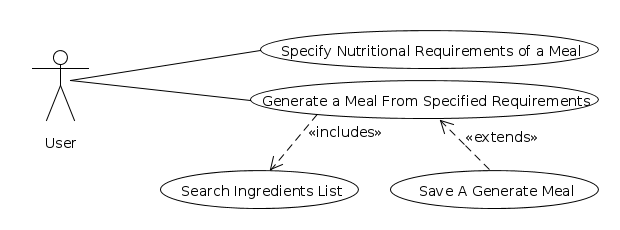
\includegraphics[width = 1\textwidth]{MealGeneration.png}
\label{useCaseDiagram:MealGeneration}
\end{figure}


%Search Ingredients Database
\begin{center}
\begin{tabularx}{\textwidth}{ |X|X|}
\hline
\multicolumn{2}{|c|}{\textbf{Search Ingredients Database}}\\
\hline
\hline
\textbf{Use Case Diagram(s)} & Figure ~\ref{useCaseDiagram:MealGeneration} \\ \hline
\textbf{Description} & User searches the ingredients database, and can review the content of ingredients.\\ \hline
\textbf{Process} & \\ \hline
\textbf{Scenarios} & \\ \hline
\textbf{Includes} & \\ \hline
\textbf{Extends} &  \\ \hline
\textbf{Pre Conditions} & \\ \hline
\textbf{Post Conditions} & \\ \hline
\textbf{Rationale} & Users may wish to view the content of an ingredient for reference or check to see if a certain brand or subtype of ingredient is in the database.\\ \hline
\end{tabularx}
\end{center}

%Specify the nutritional requirements of a meal
\begin{center}
\begin{tabularx}{\textwidth}{ |X|X|}
\hline
\multicolumn{2}{|c|}{\textbf{Specify a Meals Nutritional Requirements}}\\
\hline
\hline
\textbf{Use Case Diagram(s)} & Figure ~\ref{useCaseDiagram:MealGeneration} \\ \hline
\textbf{Description} & The requirements for a meal may be specified manually or inferred from the users daily nutritional requirements.\\ \hline
\textbf{Process} & \\ \hline
\textbf{Scenarios} & \\ \hline
\textbf{Includes} & \\ \hline
\textbf{Extends} &  \\ \hline
\textbf{Pre Conditions} & \\ \hline
\textbf{Post Conditions} & \\ \hline
\textbf{Rationale} & Requirements are needed to generate the meal, by setting the constraints over which to compute the meal.\\ \hline
\end{tabularx}
\end{center}

%Generate a meal from requirements
\begin{center}
\begin{tabularx}{\textwidth}{ |X|X|}
\hline
\multicolumn{2}{|c|}{\textbf{Generate a Meal}}\\
\hline
\hline
\textbf{Use Case Diagram(s)} & Figure ~\ref{useCaseDiagram:MealGeneration}\\ \hline
\textbf{Description} & Generate a meal from a set of specified ingredients and requirements.\\ \hline
\textbf{Process} & \\ \hline
\textbf{Scenarios} & \\ \hline
\textbf{Includes} Search Ingredients Database; Specify a Meals Nutritional Requirements. & \\ \hline
\textbf{Extends} &  \\ \hline
\textbf{Pre Conditions} & \\ \hline
\textbf{Post Conditions} & \\ \hline
\textbf{Rationale} & Meal generation is the key feature of the project.\\ \hline
\end{tabularx}
\end{center}


%Save a generated meal
\begin{center}
\begin{tabularx}{\textwidth}{ |X|X|}
\hline
\multicolumn{2}{|c|}{\textbf{Save a Generated Meal}}\\
\hline
\hline
\textbf{Use Case Diagram(s)} & Figure ~\ref{useCaseDiagram:MealGeneration}\\ \hline
\textbf{Description} & Save a generated meal to be used at a later date.\\ \hline
\textbf{Process} & \\ \hline
\textbf{Scenarios} & \\ \hline
\textbf{Includes} & \\ \hline
\textbf{Extends} & Generate a Meal  \\ \hline
\textbf{Pre Conditions} & An unsaved meal has been generated.\\ \hline
\textbf{Post Conditions} & Meal is saved to user's account.\\ \hline
\textbf{Rationale} & Nutritional requirements are needed to generate satisfactory meals.\\ \hline
\end{tabularx}
\end{center}



\end{document}

